% ============================================================
\section{Resultados y Discusión}
% ============================================================

\subsection{Caso A: Entrenamiento e Inferencia del Modelo Ajustado}
\label{sec:res_a}

La Tabla~\ref{tab:epochs} contrasta la primera y la última época del
entrenamiento en GPU. La caída simultánea de las tres pérdidas principales y el
incremento de mAP50 de cajas desde 0.192 hasta 0.792 confirman una convergencia
sana, sin señales de sobreajuste dentro de la paciencia configurada.

\begin{table}[H]
\centering
\caption{Evolución del entrenamiento de YOLO26n-seg (Tesla T4, 60 épocas).}
\label{tab:epochs}
\setlength{\tabcolsep}{6pt}
\begin{tabular}{lcc}
  \toprule
  \textbf{Métrica} & \textbf{Época 1/60} & \textbf{Época 60/60} \\
  \midrule
  VRAM ocupada (\texttt{GPU\_mem})    & 3.31\,GiB & 4.60\,GiB \\
  \texttt{box\_loss}                  & 0.8241    & 0.5509 \\
  \texttt{seg\_loss}                  & 1.9250    & 0.7458 \\
  \texttt{cls\_loss}                  & 4.5030    & 0.4008 \\
  Box: precisión / recall             & 0.539 / 0.189 & 0.897 / 0.691 \\
  Box: mAP50 / mAP50-95               & 0.192 / 0.137 & 0.792 / 0.695 \\
  Mask: mAP50 / mAP50-95              & 0.151 / 0.069 & 0.792 / 0.606 \\
  Tiempo de la época                  & 1\,min\,28\,s + 31\,s val. & 55.4\,s + 5.5\,s val. \\
  \bottomrule
\end{tabular}
\end{table}

En tiempo total, las 60 épocas en la Tesla T4 (a un promedio de
$\approx$1\,min\,30\,s por época) sumaron \textbf{$\approx$90 minutos},
frente a las \textbf{3.5--4 horas} que tomó el mismo entrenamiento sobre la CPU
Xeon de 2 vCPU del entorno, es decir, una aceleración de
\textbf{2.4--2.7$\times$} incluso contra una GPU de gama de inferencia como la
T4 y con un dataset que satura el pipeline de datos. Cabe señalar que durante
el entrenamiento en CPU el proceso Python se mantuvo clavado en 87--100\,\% de
uso de procesador, mientras que en GPU la CPU quedó libre para el pipeline de
carga de imágenes.

La matriz de confusión del modelo final (Figura~\ref{fig:confusion}) muestra
diagonales dominantes en las cuatro clases (332 aciertos en \textit{hammer},
177 en \textit{wrench}, 155 en \textit{screw}); el principal modo de error es
la confusión con el fondo (58, 42 y 27 instancias respectivamente), típico de
objetos delgados como tornillos y llaves.

\begin{figure}[H]
  \centering
  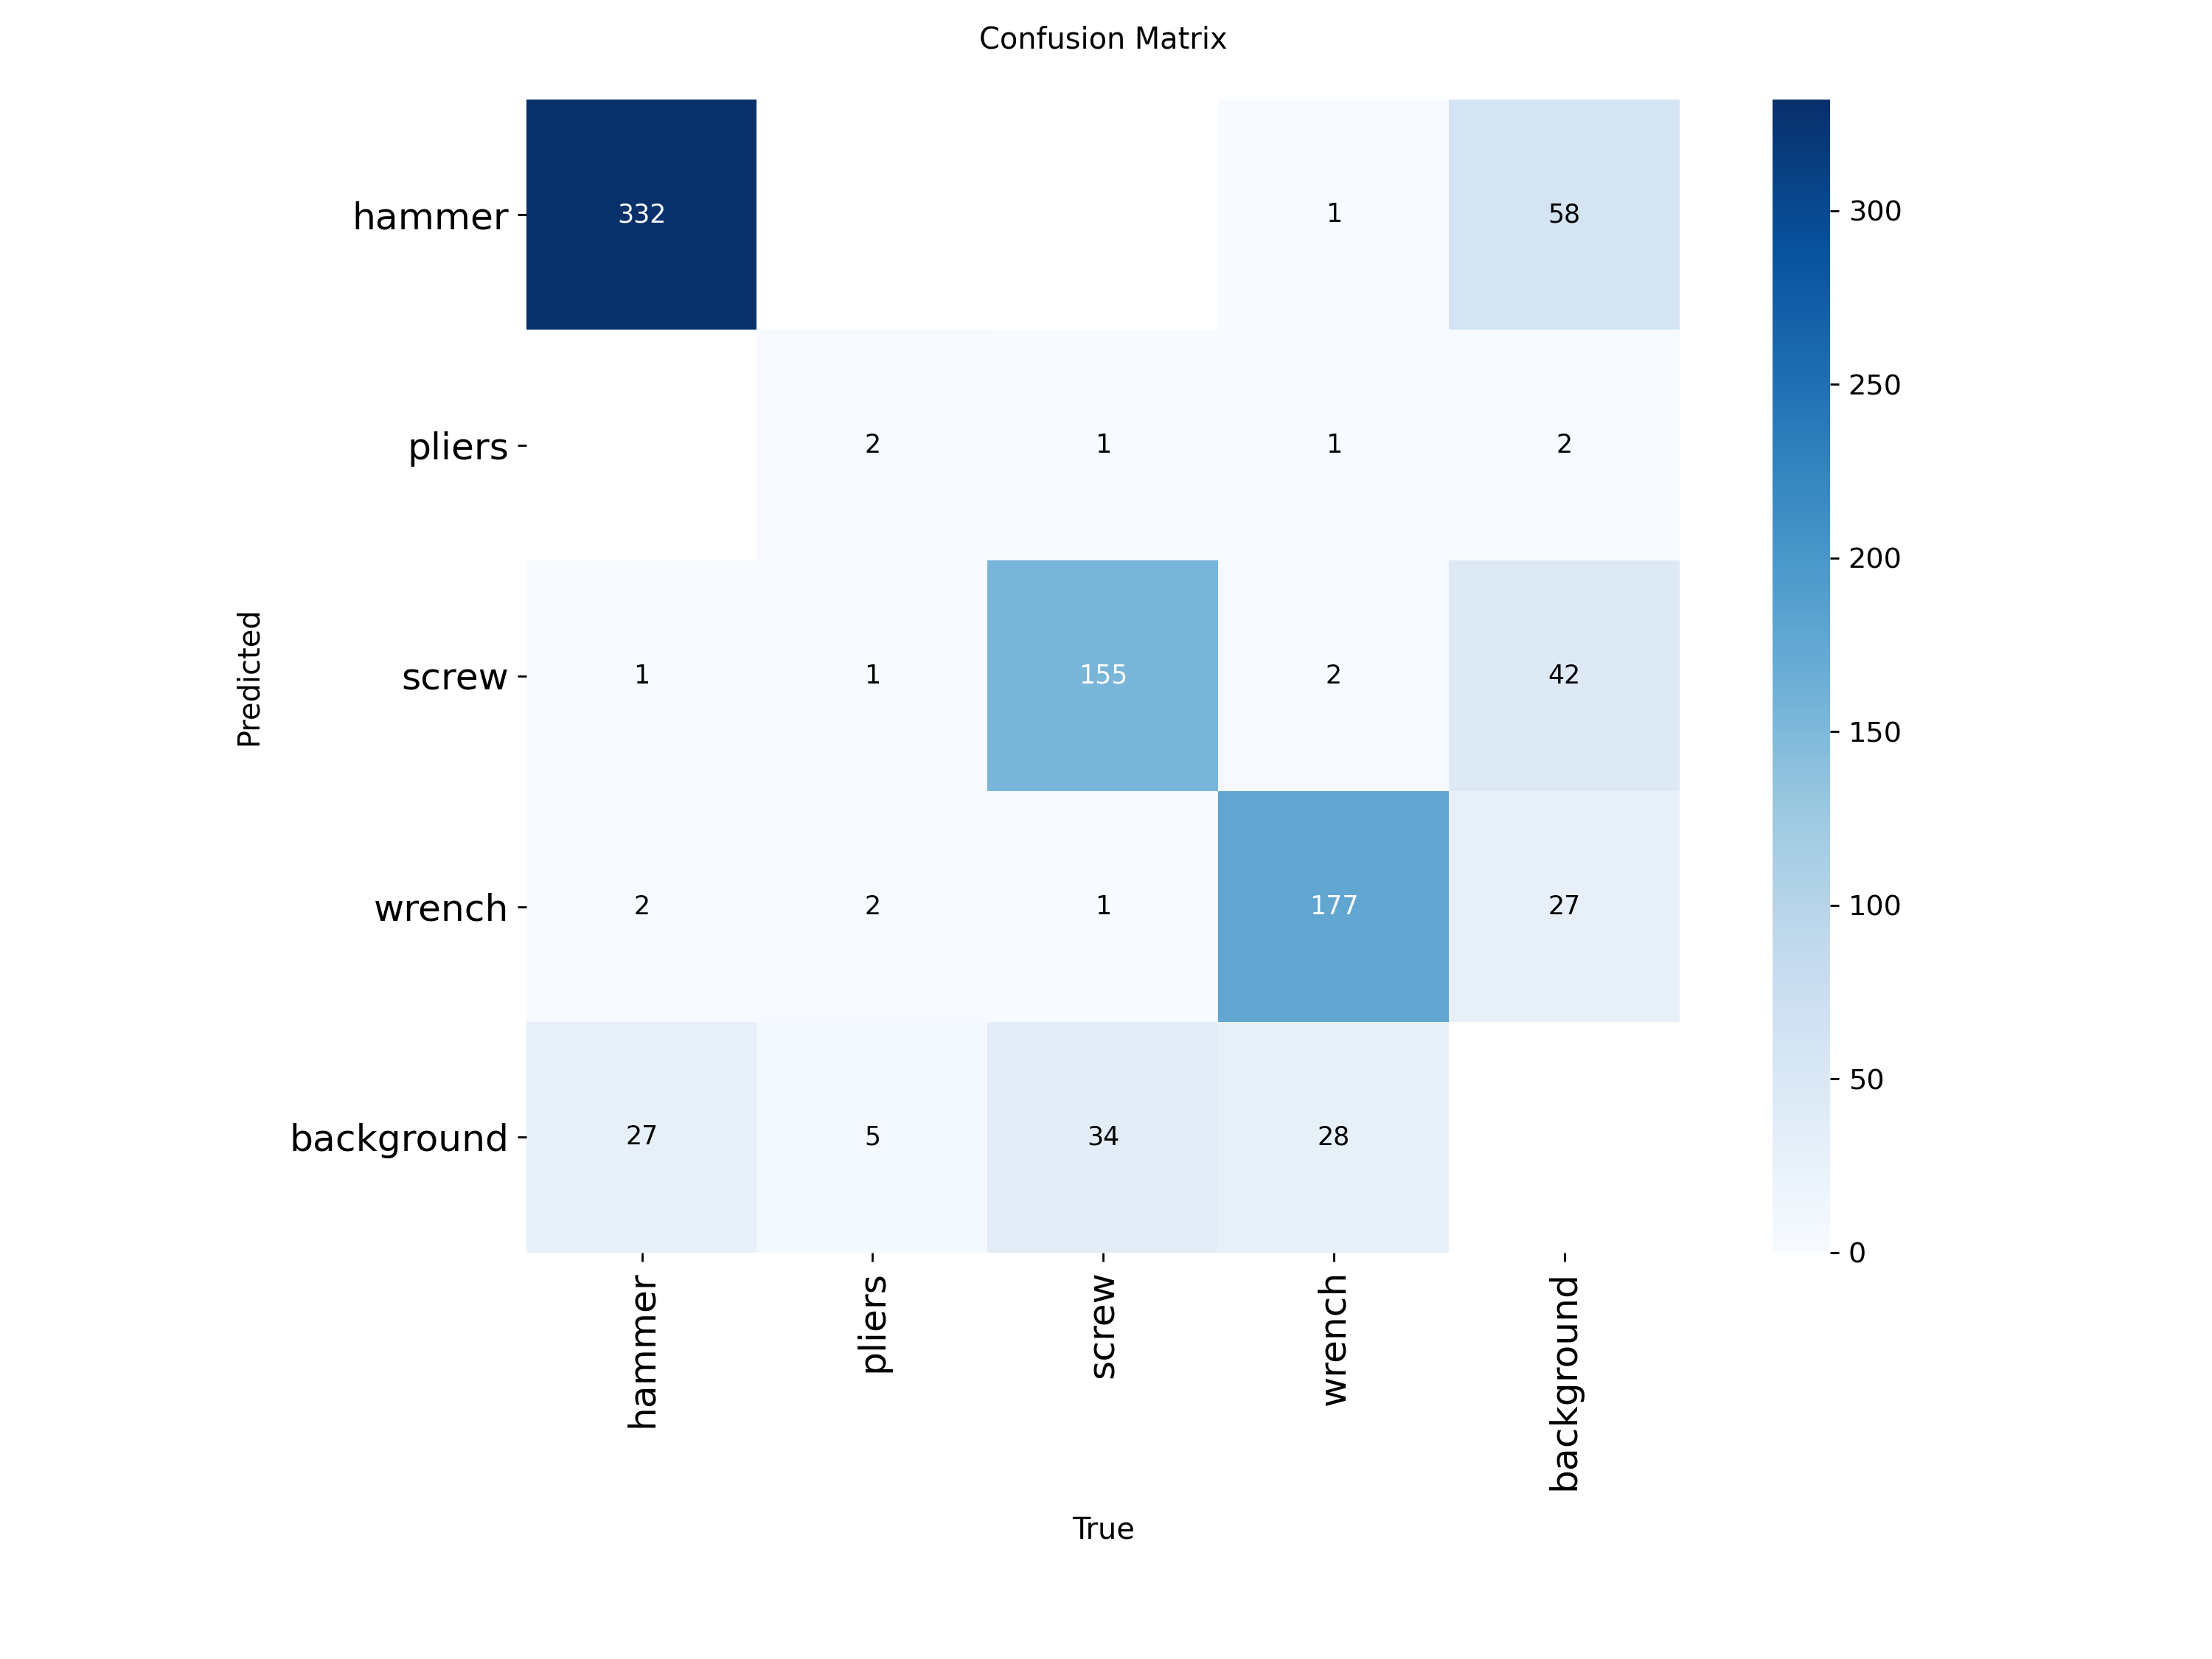
\includegraphics[width=0.8\textwidth]{imagenes/sectionA/matriz_confusion.png}
  \caption{Matriz de confusión del modelo YOLO26n-seg ajustado sobre el
           conjunto de validación (4 clases + fondo).}
  \label{fig:confusion}
\end{figure}

En la evaluación local (CPU del equipo de desarrollo) sobre el subconjunto de
test exportado, las métricas descienden (mAP50 $= 0.295$, precisión $= 0.619$,
recall $= 0.261$; Figura~\ref{fig:metricas_eval}), lo que se atribuye al cambio
de dominio de las imágenes locales respecto al conjunto de Roboflow. El tiempo
medio de predicción en CPU fue de \textbf{98.6\,ms por imagen}
(Figura~\ref{fig:tiempo_cpu}), equivalente a $\approx$10 FPS teóricos, cifra
coherente con los \textbf{10.9 FPS} medidos con la cámara web en vivo
(Figura~\ref{fig:inferencia_local}).

\begin{figure}[H]
  \centering
  \begin{subfigure}[b]{0.55\textwidth}
    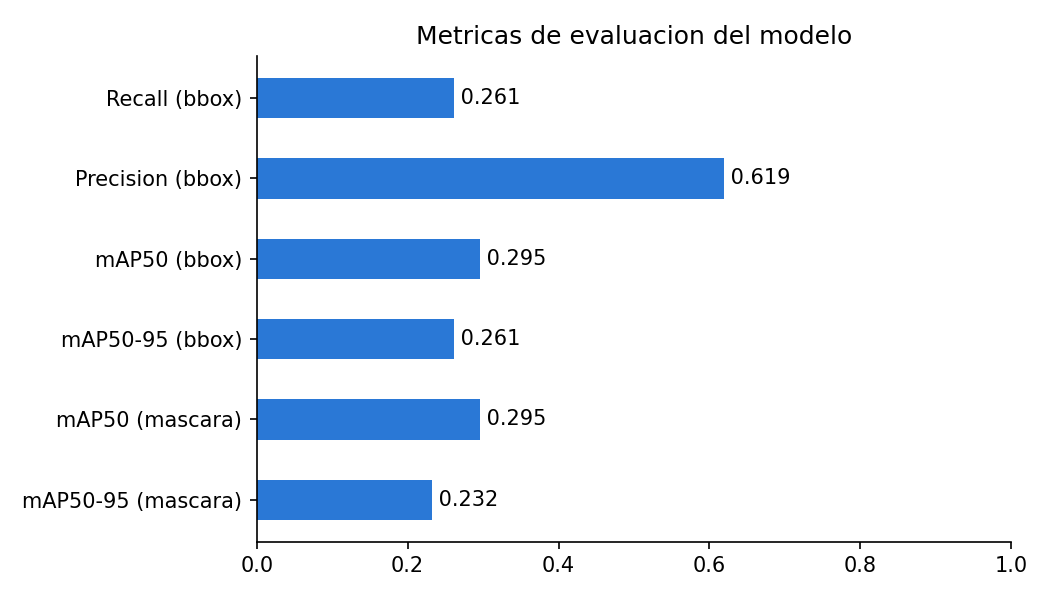
\includegraphics[width=\textwidth]{imagenes/sectionA/metricas_evaluacion.png}
    \caption{Métricas de la evaluación local.}
    \label{fig:metricas_eval}
  \end{subfigure}\hfill
  \begin{subfigure}[b]{0.42\textwidth}
    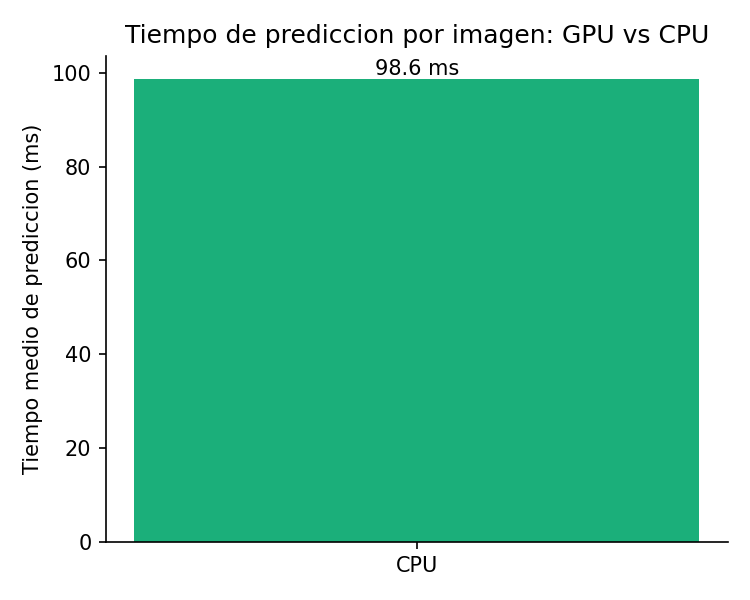
\includegraphics[width=\textwidth]{imagenes/sectionA/tiempo_prediccion_gpu_vs_cpu.png}
    \caption{Tiempo medio de predicción (CPU): 98.6\,ms.}
    \label{fig:tiempo_cpu}
  \end{subfigure}
  \caption{Evaluación del modelo ajustado en el equipo local (inferencia CPU).}
  \label{fig:eval_local}
\end{figure}

\begin{figure}[H]
  \centering
  \begin{subfigure}[b]{0.55\textwidth}
    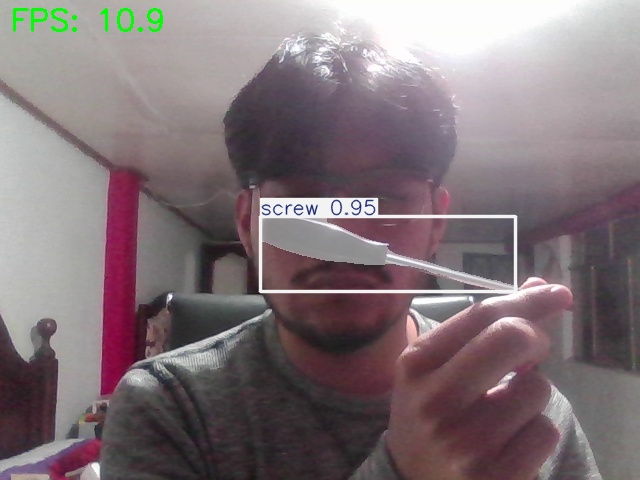
\includegraphics[width=\textwidth]{imagenes/sectionA/yolo_camara.jpg}
    \caption{Cámara web en vivo: \textit{screw} 0.95 a 10.9 FPS (CPU).}
  \end{subfigure}\hfill
  \begin{subfigure}[b]{0.42\textwidth}
    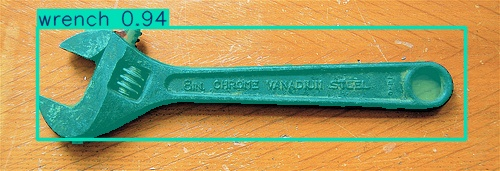
\includegraphics[width=\textwidth]{imagenes/sectionA/yolo_imagen.JPEG}
    \caption{Imagen estática: \textit{wrench} 0.94.}
  \end{subfigure}
  \caption{Inferencia local del modelo YOLO26n-seg ajustado.}
  \label{fig:inferencia_local}
\end{figure}

\subsection{Caso B: YOLOv12n vs.\ YOLO26n y Real-ESRGAN}
\label{sec:res_b}

La Figura~\ref{fig:yolo_fps} recoge las cuatro corridas sobre el mismo video en
la estación del laboratorio. Los FPS superpuestos en pantalla y el estado de
\texttt{btop} en cada captura resumen el comportamiento: en CPU, ambos modelos
reparten la carga entre los 24 hilos del i9-12900K (núcleos entre 27 y 84\,\%,
reloj a 4.9\,GHz, 67--70\,$^{\circ}$C) con la GPU ociosa (1\,\%, 436\,MiB de
base); en CUDA, la situación se invierte: la CPU cae a 6--7\,\% con el reloj
reducido a 0.8--1.3\,GHz y la VRAM sube a 743\,MiB.

\begin{figure}[H]
  \centering
  \begin{subfigure}[b]{0.49\textwidth}
    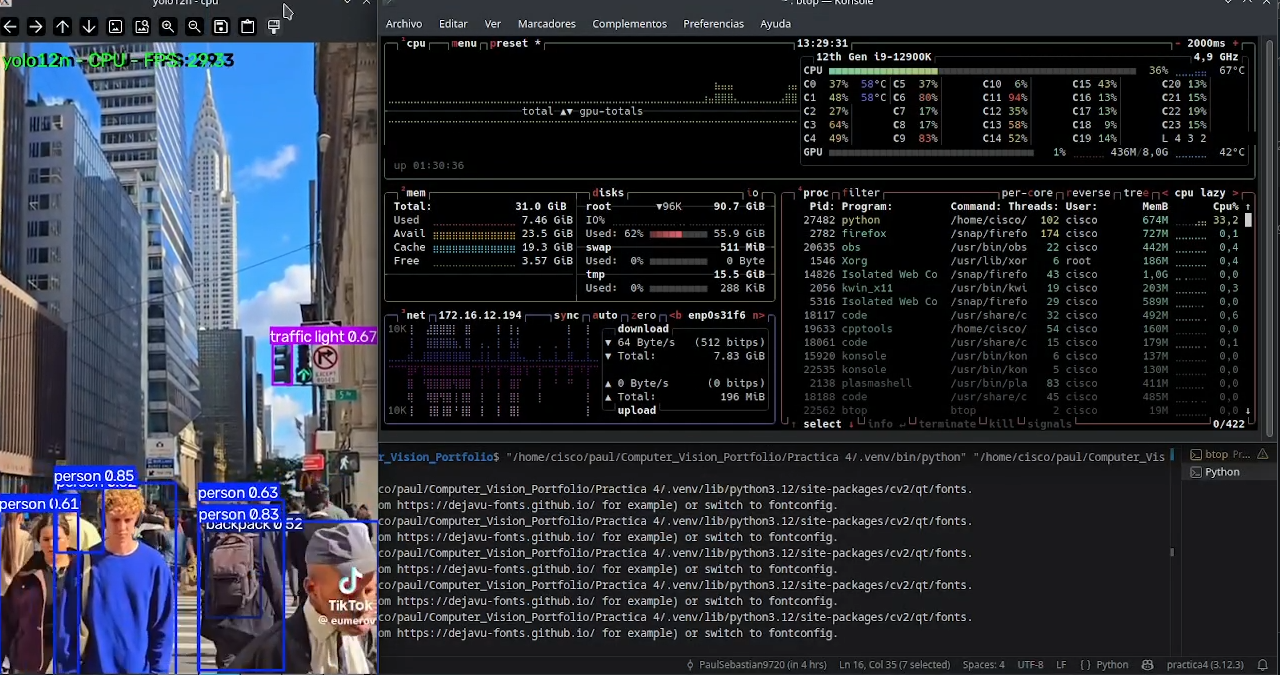
\includegraphics[width=\textwidth]{imagenes/sectionB/yolo/cpu_yolo12.png}
    \caption{YOLOv12n en CPU: 29.3 FPS.}
  \end{subfigure}\hfill
  \begin{subfigure}[b]{0.49\textwidth}
    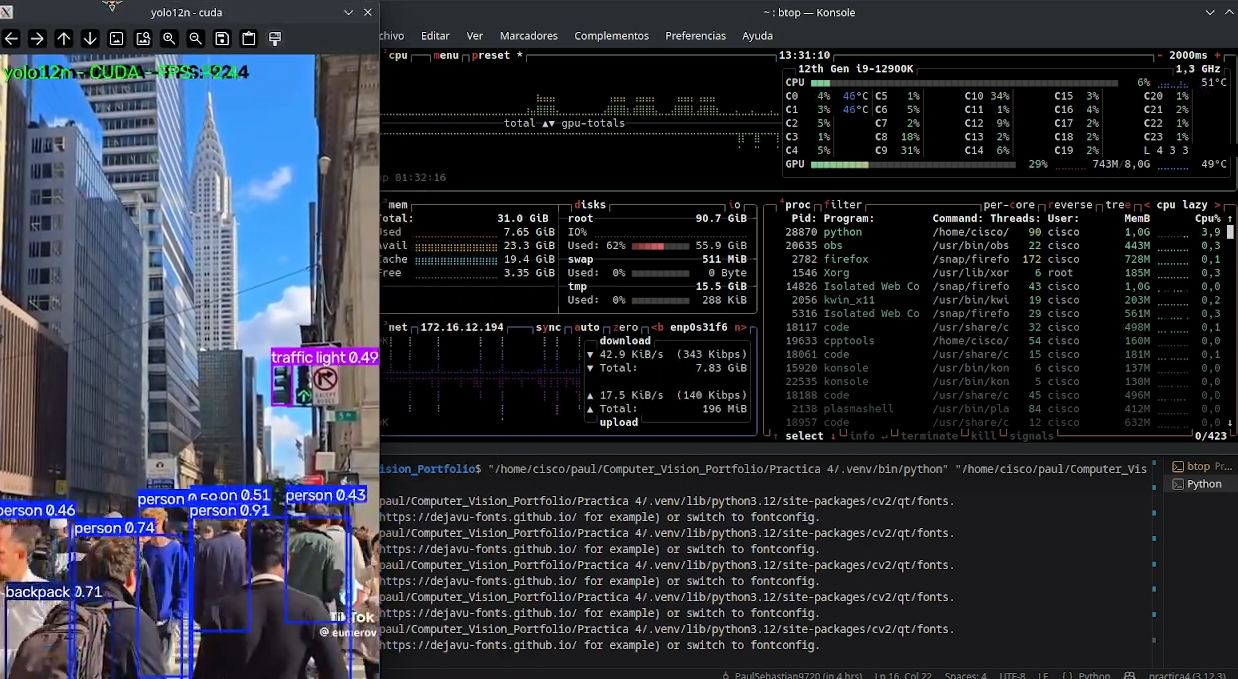
\includegraphics[width=\textwidth]{imagenes/sectionB/yolo/gpu_yolo12.png}
    \caption{YOLOv12n en CUDA: 122.4 FPS.}
  \end{subfigure}\\[0.6em]
  \begin{subfigure}[b]{0.49\textwidth}
    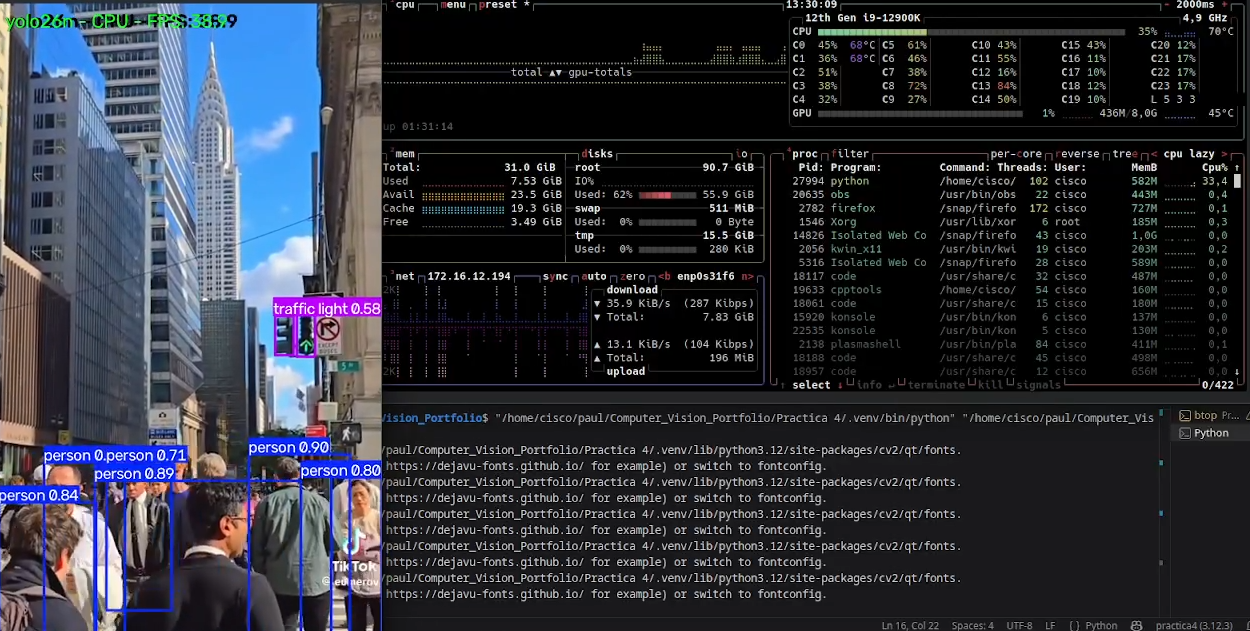
\includegraphics[width=\textwidth]{imagenes/sectionB/yolo/cpu_yolo26.png}
    \caption{YOLO26n en CPU: 38.9 FPS.}
  \end{subfigure}\hfill
  \begin{subfigure}[b]{0.49\textwidth}
    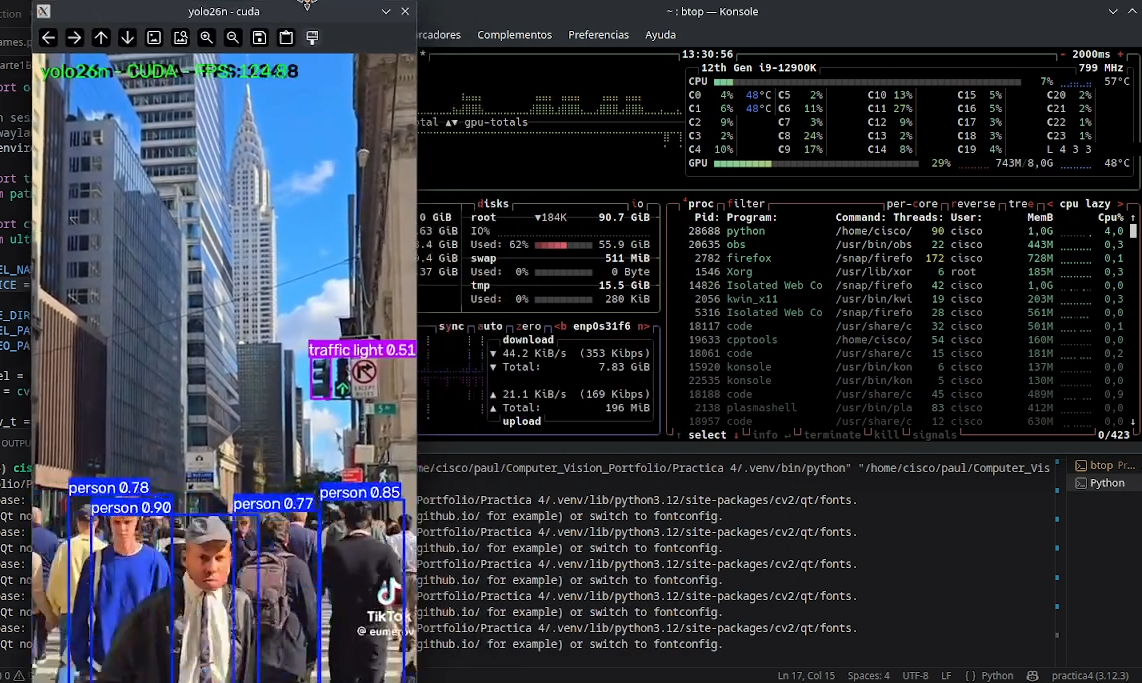
\includegraphics[width=\textwidth]{imagenes/sectionB/yolo/gpu_yolo26.png}
    \caption{YOLO26n en CUDA: 124.8 FPS.}
  \end{subfigure}
  \caption{Inferencia sobre video con dos variantes YOLO en la estación del
           laboratorio (i9-12900K / RTX 3070), con monitoreo \texttt{btop}
           simultáneo.}
  \label{fig:yolo_fps}
\end{figure}

\begin{table}[H]
\centering
\caption{FPS medidos por modelo y dispositivo (video \texttt{personas.mp4}).}
\label{tab:yolo_fps}
\begin{tabular}{lccc}
  \toprule
  \textbf{Modelo} & \textbf{CPU (FPS)} & \textbf{GPU (FPS)} & \textbf{Speedup} \\
  \midrule
  YOLOv12n & 29.3 & 122.4 & 4.2$\times$ \\
  YOLO26n  & 38.9 & 124.8 & 3.2$\times$ \\
  \bottomrule
\end{tabular}
\end{table}

Dos observaciones se desprenden de la Tabla~\ref{tab:yolo_fps}. Primera: en
CPU, YOLO26n supera a YOLOv12n (38.9 vs.\ 29.3 FPS), reflejo de las
optimizaciones de arquitectura de la generación más reciente. Segunda: en GPU
ambos modelos convergen a $\approx$122--125 FPS, señal de que la inferencia
deja de ser el cuello de botella y el límite pasa a estar en las etapas de CPU
del bucle (decodificación del video, anotación del cuadro y visualización). En
ese régimen, la GPU queda parcialmente ociosa esperando cuadros.

En Real-ESRGAN la brecha es cualitativamente mayor
(Figura~\ref{fig:esrgan_frames}): el recorte de $160\times160$ ampliado
$\times$4 corre a \textbf{0.36 FPS en CPU} frente a \textbf{1.57 FPS en CUDA};
en la modalidad de cuadro completo muestreado cada 2\,s, los tiempos fueron
4.40\,s (CPU) frente a 1.12\,s (GPU), un speedup de \textbf{3.9$\times$}. El
costo sistémico de la vía CPU es notable (Figura~\ref{fig:esrgan_btop}): 52\,\%
de uso agregado de los 24 hilos con picos de \textbf{91\,$^{\circ}$C} a
4.9\,GHz, mientras que en CUDA la GPU trabaja al 62\,\% con 899\,MiB de VRAM y
la CPU desciende a 5\,\% (44\,$^{\circ}$C).

\begin{figure}[H]
  \centering
  \begin{subfigure}[b]{0.49\textwidth}
    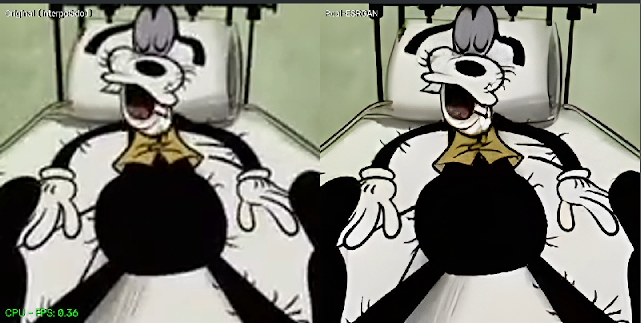
\includegraphics[width=\textwidth]{imagenes/sectionB/mejora/cpu_frame_1.png}
    \caption{CPU: 0.36 FPS.}
  \end{subfigure}\hfill
  \begin{subfigure}[b]{0.49\textwidth}
    
\includegraphics[width=\textwidth]{imagenes/sectionB/mejora/gpu_frame_1.png}
    \caption{CUDA: 1.57 FPS.}
  \end{subfigure}
  \caption{Real-ESRGAN x4plus sobre recorte central (original interpolado
           vs.\ superresolución).}
  \label{fig:esrgan_frames}
\end{figure}

\begin{figure}[H]
  \centering
  \begin{subfigure}[b]{0.49\textwidth}
    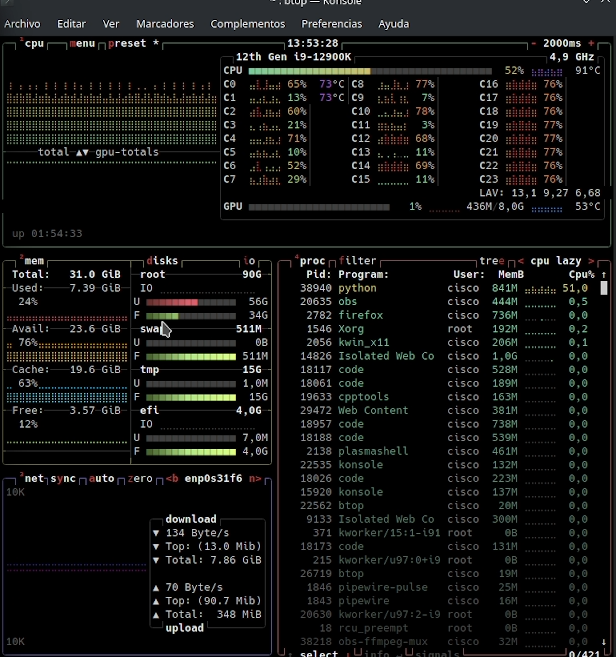
\includegraphics[width=\textwidth]{imagenes/sectionB/mejora/cpu_frame_1_btop.png}
    \caption{Modo CPU: 52\,\% agregado, 4.9\,GHz, 91\,$^{\circ}$C; GPU 1\,\%.}
  \end{subfigure}\hfill
  \begin{subfigure}[b]{0.49\textwidth}
    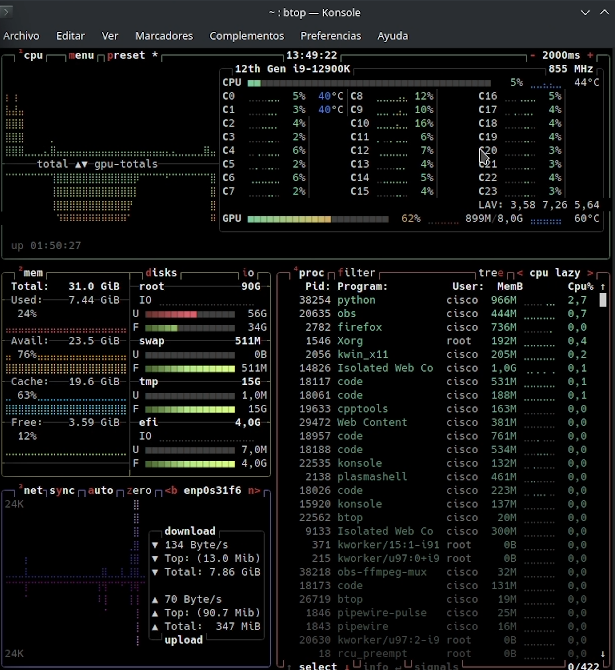
\includegraphics[width=\textwidth]{imagenes/sectionB/mejora/gpu_frame_1_btop.png}
    \caption{Modo CUDA: GPU 62\,\%, 899\,MiB VRAM; CPU 5\,\%.}
  \end{subfigure}
  \caption{Monitoreo \texttt{btop} durante Real-ESRGAN: la carga migra por
           completo de la CPU a la GPU.}
  \label{fig:esrgan_btop}
\end{figure}

\subsection{Caso C: Pipeline de Bordes en C++}
\label{sec:res_c}

Las Figuras~\ref{fig:bordes_cpu} y~\ref{fig:bordes_gpu} muestran ambos
ejecutables procesando video con el HUD de tiempo por cuadro: la versión CPU
promedia \textbf{6.666\,ms/cuadro (150 FPS)} y la versión GPU-only
\textbf{2.314\,ms/cuadro (432 FPS)}, es decir, un speedup de
\textbf{2.9$\times$}. Durante la corrida GPU, \texttt{nvidia-smi}
(Figura~\ref{fig:nvidia_smi_c}) reporta al proceso
\texttt{./build/preprocesamiento\_gpu} con apenas \textbf{172\,MiB de VRAM},
utilización del \textbf{2\,\%} y 47\,W sobre un límite de 220\,W.

\begin{figure}[H]
  \centering
  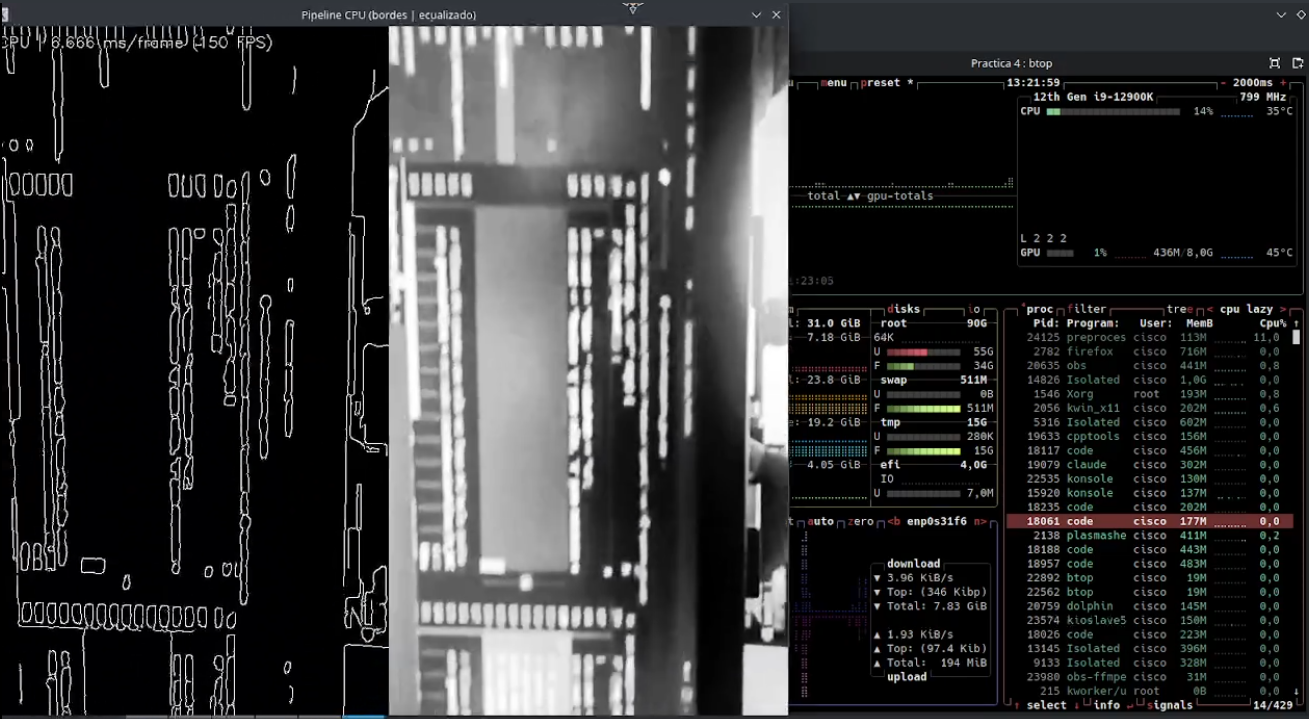
\includegraphics[width=0.95\textwidth]{imagenes/sectionC/bordes_cpu1.png}
  \caption{Pipeline CPU (bordes\,$|$\,ecualizado): 6.666\,ms/cuadro (150 FPS);
           \texttt{btop} registra 14\,\% de CPU y GPU ociosa (1\,\%).}
  \label{fig:bordes_cpu}
\end{figure}

\begin{figure}[H]
  \centering
  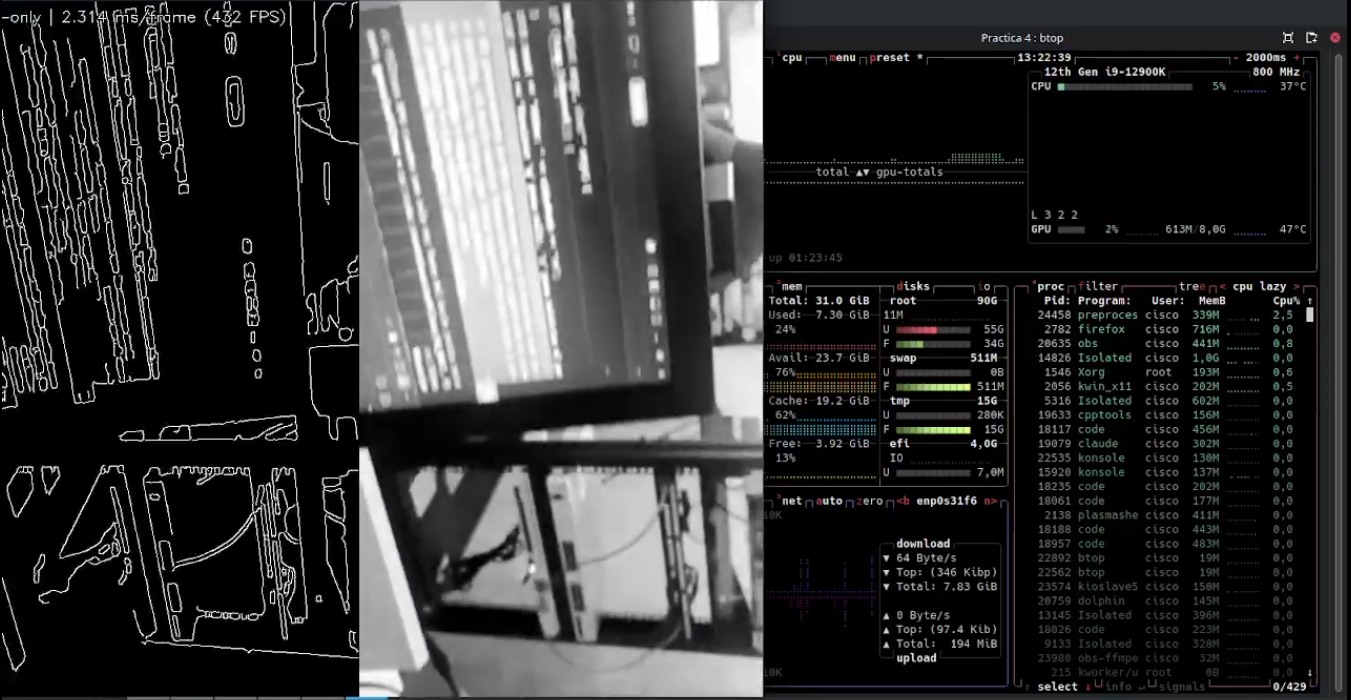
\includegraphics[width=0.95\textwidth]{imagenes/sectionC/bordes_gpu1.png}
  \caption{Pipeline GPU-only: 2.314\,ms/cuadro (432 FPS); el uso de CPU cae a
           5\,\% y la VRAM sube a 613\,MiB totales del sistema.}
  \label{fig:bordes_gpu}
\end{figure}

\begin{figure}[H]
  \centering
  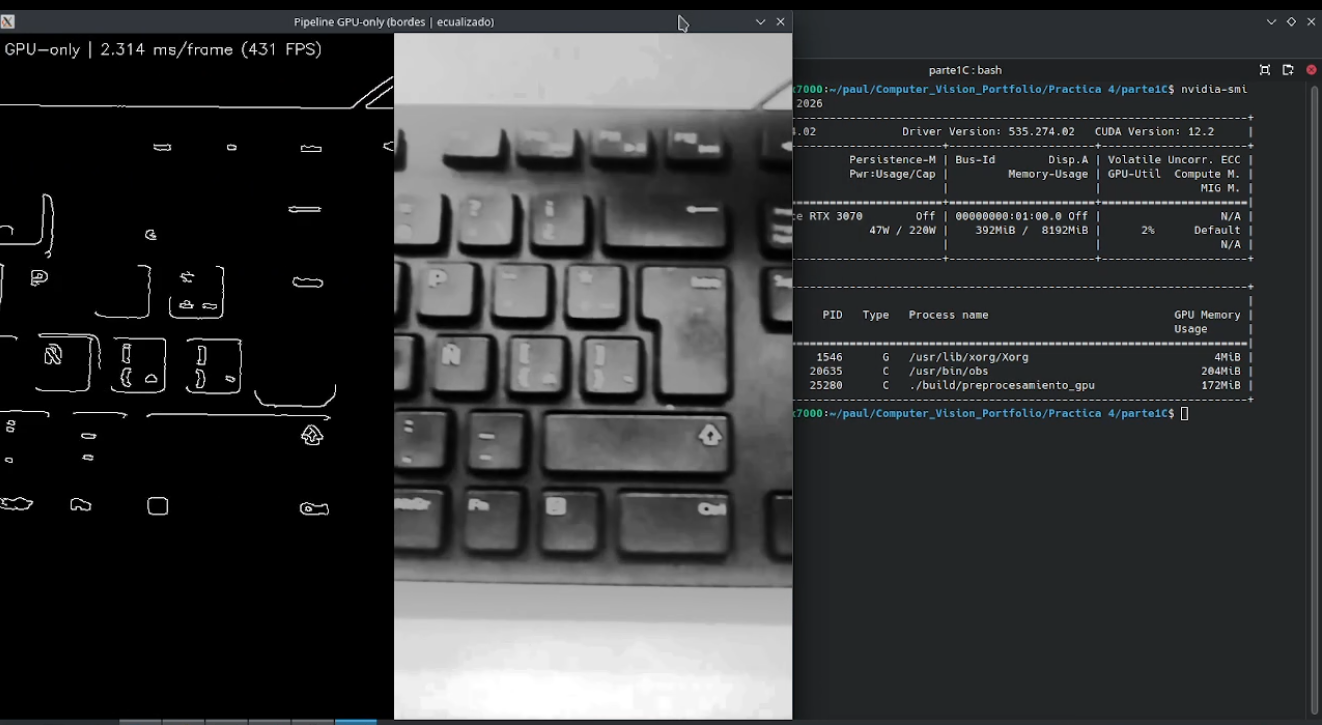
\includegraphics[width=0.95\textwidth]{imagenes/sectionC/gpu_nvidia_smi.png}
  \caption{\texttt{nvidia-smi} durante la corrida GPU del caso C: RTX 3070 al
           2\,\% de utilización, 47\,W/220\,W, con el proceso
           \texttt{preprocesamiento\_gpu} ocupando 172\,MiB de VRAM.}
  \label{fig:nvidia_smi_c}
\end{figure}

\subsection{Cuadro Comparativo Global y Discusión}

\begin{table}[H]
\centering
\caption{Resumen comparativo CPU vs.\ GPU de los tres casos de prueba.}
\label{tab:global}
\setlength{\tabcolsep}{4.5pt}
\small
\begin{tabular}{llccc}
  \toprule
  \textbf{Caso} & \textbf{Carga} & \textbf{CPU} & \textbf{GPU} & \textbf{Speedup} \\
  \midrule
  A & Entrenamiento YOLO26n-seg (60 ép.) & 3.5--4\,h & $\approx$90\,min & 2.4--2.7$\times$ \\
  A & Inferencia local (imagen)          & 98.6\,ms  & ---              & --- \\
  B & YOLOv12n video                     & 29.3 FPS  & 122.4 FPS        & 4.2$\times$ \\
  B & YOLO26n video                      & 38.9 FPS  & 124.8 FPS        & 3.2$\times$ \\
  B & Real-ESRGAN (cuadro completo)      & 4.40\,s   & 1.12\,s          & 3.9$\times$ \\
  B & Real-ESRGAN (recorte en vivo)      & 0.36 FPS  & 1.57 FPS         & 4.4$\times$ \\
  C & Bordes C++ OpenCV                  & 6.67\,ms (150 FPS) & 2.31\,ms (432 FPS) & 2.9$\times$ \\
  \bottomrule
\end{tabular}
\end{table}

\begin{table}[H]
\centering
\caption{Consumo de recursos observado durante las pruebas.}
\label{tab:recursos}
\setlength{\tabcolsep}{4.5pt}
\small
\begin{tabular}{llll}
  \toprule
  \textbf{Prueba} & \textbf{CPU (\%) / temp.} & \textbf{RAM} & \textbf{VRAM} \\
  \midrule
  A entren.\ GPU (T4)      & pipeline de datos       & 6.3\,GiB usados & 3.31--4.6\,GiB \\
  A entren.\ CPU (Xeon)    & 87--100\,\% / ---       & 5.2\,GiB proc.\ & --- \\
  B YOLO modo CPU          & núcleos 27--84\,\% / 67--70\,$^{\circ}$C & 7.5\,GiB & 436\,MiB (base) \\
  B YOLO modo CUDA         & 6--7\,\% / 51\,$^{\circ}$C  & 7.65\,GiB & 743\,MiB \\
  B ESRGAN modo CPU        & 52\,\% agreg.\ / 91\,$^{\circ}$C & 7.39\,GiB & 436\,MiB (base) \\
  B ESRGAN modo CUDA       & 5\,\% / 44\,$^{\circ}$C     & 7.44\,GiB & 899\,MiB \\
  C bordes modo CPU        & 14\,\% / 35\,$^{\circ}$C    & 7.18\,GiB & 436\,MiB (base) \\
  C bordes modo GPU        & 5\,\% / 37\,$^{\circ}$C     & 7.30\,GiB & 613\,MiB (172 del proceso) \\
  \bottomrule
\end{tabular}
\end{table}

\paragraph{¿Por qué gana la GPU en cada caso, y por cuánto?}
Los tres casos ilustran regímenes distintos de la misma ley: el speedup depende
de la razón entre cómputo paralelizable y costo de transferencia.

\begin{itemize}
  \item \textbf{Caso A (entrenamiento).} El entrenamiento es el escenario más
        favorable a la GPU: convoluciones y retropropagación son
        multiplicaciones matriciales masivas que saturan los SM, y el dataset
        reside en VRAM por lotes. El speedup observado (2.4--2.7$\times$)
        está acotado por la modestia de la T4 y por el pipeline de datos
        (decodificación JPEG y aumentos corren en una CPU de solo 2 vCPU); con
        una CPU anfitriona más capaz el margen crecería.
  \item \textbf{Caso B (inferencia profunda).} En redes convolucionales de
        inferencia el cómputo por cuadro sigue dominando sobre la
        transferencia de un único cuadro, de ahí los 3.2--4.4$\times$. El
        techo común de $\approx$125 FPS de ambas YOLO en GPU demuestra el
        efecto Amdahl: acelerada la red, mandan las etapas secuenciales de CPU
        (decodificación y dibujo). Real-ESRGAN, con 23 bloques residuales
        sobre cada píxel, es directamente inviable en CPU para uso interactivo
        (0.36 FPS y 91\,$^{\circ}$C sostenidos).
  \item \textbf{Caso C (procesamiento clásico).} Filtros gaussianos,
        morfología y Canny son operaciones de baja intensidad aritmética
        (memoria-limitadas). Aun así la GPU logra 2.9$\times$ porque el
        pipeline mantiene los datos en VRAM entre etapas (una sola subida y
        una sola bajada por cuadro); si cada operación viajara por PCIe, la
        latencia de transferencia anularía la ganancia. La utilización del
        2\,\% en \texttt{nvidia-smi} confirma que los kernels terminan casi
        instantáneamente y el tiempo restante es transferencia y
        sincronización: la GPU está sobredimensionada para esta carga.
\end{itemize}

\paragraph{Recomendaciones de uso.}
(i)~Entrenar y afinar redes profundas siempre en GPU; la CPU solo es admisible
para pruebas de humo. (ii)~Para inferencia en video con modelos nano, una CPU
de gama alta alcanza tiempo real ($\approx$30--39 FPS), por lo que la GPU se
justifica cuando se requieren múltiples flujos, modelos mayores o menor consumo
energético y térmico. (iii)~Para superresolución u otras redes generativas, la
GPU es obligatoria en cualquier escenario práctico. (iv)~En preprocesamiento
clásico, migrar a CUDA solo si el pipeline encadena varias etapas en VRAM y la
resolución o el número de flujos lo exige; a $480$p una CPU moderna ya excede
el tiempo real con amplio margen.
